\documentclass[conference]{IEEEtran}
\IEEEoverridecommandlockouts
\usepackage[utf8]{inputenc}
\usepackage[T1]{fontenc}
\usepackage[spanish,es-noshorthands,es-tabla,es-nodecimaldot]{babel}
\usepackage{amsmath,amssymb}
\usepackage{graphicx}
\usepackage{booktabs}
\usepackage{url}
\usepackage[hidelinks]{hyperref}
\graphicspath{{figures/}}

\begin{document}

\title{Predicción del nivel relativo de comisiones del siguiente bloque de Bitcoin mediante aprendizaje supervisado}

\author{
\IEEEauthorblockN{Carlos David Ordinola Ortega, Nayeli Belén Guerrero Gutierrez, Adriana Celeste Alvarado León}
\IEEEauthorblockA{Universidad de Ingeniería y Tecnología (UTEC), Lima, Perú\\
Machine Learning (CS3061) --- 2026-2}
}

\maketitle

\begin{abstract}
En Bitcoin, el espacio de cada bloque es limitado y las transacciones compiten mediante comisiones. Este trabajo plantea una clasificación binaria a nivel de bloque: anticipar si la tasa mediana de comisión del bloque siguiente superará el percentil 75 de las 1008 tasas más recientes, usando solo información disponible hasta el bloque actual. Se emplean 418\,720 bloques de 2016 a 2023 del conjunto \textit{Bitcoin Blockchain Historical Data}, con una partición cronológica 70/15/15. Se comparan una referencia de persistencia, una regresión logística regularizada, Random Forest e HistGradientBoosting, con selección temporal de hiperparámetros y del umbral de decisión. En prueba, RF y HGB alcanzan F1 de 0.605 y 0.609, frente a 0.576 de la persistencia y 0.570 de la regresión logística; sus precisiones promedio son 0.684 y 0.690. En validación, los modelos de árboles alcanzan un F1 de 0.564--0.571 y una precisión promedio de 0.62--0.63, frente a 0.540 y 0.593 de las referencias. Un estudio de ablación muestra que la ganancia procede de la historia reciente de las comisiones (+0.088 de precisión promedio), mientras que la actividad de la red aporta poco (+0.007) y el calendario nada. El análisis de errores indica que los modelos fallan sobre todo al inicio de los episodios de comisión alta, que duran en promedio unos dos bloques, lo que apunta a la ausencia de información del \textit{mempool} como límite principal.
\end{abstract}

\begin{IEEEkeywords}
Bitcoin, comisiones, clasificación binaria, series temporales, ensambles de árboles, estudio de ablación
\end{IEEEkeywords}

% =====================================================================
\section{Introducción}
Bitcoin es una red de pagos descentralizada en la que las transacciones se agrupan en bloques que se minan, en promedio, cada diez minutos. Cada bloque tiene una capacidad limitada, por lo que la inclusión de una transacción no está garantizada: los mineros seleccionan las transacciones que les resultan más rentables, es decir, las que ofrecen una comisión mayor por unidad de espacio. Cuando la demanda supera la capacidad disponible, se forma una subasta implícita en la que los usuarios compiten ofreciendo comisiones más altas.

Esta dinámica convierte la elección de la comisión en una decisión con costo en ambos sentidos. Una comisión insuficiente puede dejar la transacción sin confirmar durante horas; una excesiva constituye un sobrecosto irrecuperable, dado que las transacciones son irreversibles. Las carteras incorporan estimadores de comisión, pero su desempeño es limitado precisamente en los episodios de congestión, que son aquellos en los que una estimación correcta resulta más valiosa.

El objetivo de este trabajo es determinar si, a partir del estado observable de la red hasta el bloque actual, es posible anticipar si la comisión del siguiente bloque será \emph{alta respecto al nivel vigente del mercado}. El resultado no constituye un estimador de comisión completo, sino su primer componente: la estimación del nivel de precio, sobre la cual un estimador operativo aplicaría después la urgencia de cada usuario.

La primera etapa del proyecto formuló el problema, delimitó el periodo de estudio y diseñó la variable objetivo. Esta segunda etapa desarrolla el preprocesamiento, compara cuatro métodos con un protocolo temporal común y analiza en qué condiciones funcionan y por qué fallan. Las contribuciones son: (i) una comparación de persistencia, regresión logística, Random Forest e HistGradientBoosting bajo las mismas particiones cronológicas; (ii) un estudio de ablación que cuantifica el aporte de cada grupo de variables con intervalos de confianza que respetan la dependencia temporal; y (iii) un análisis de errores que identifica el inicio de los episodios de congestión como la principal fuente de fallo.

% =====================================================================
\section{Trabajos relacionados}
El mercado de comisiones de Bitcoin se ha estudiado principalmente desde la economía. Möser y Böhme \cite{moser2015} analizaron la evolución longitudinal de las comisiones y mostraron que, durante los primeros años, estaban determinadas sobre todo por los valores por defecto del software cliente y no por la competencia entre usuarios. Easley, O'Hara y Basu \cite{easley2019} estudiaron cómo las comisiones pasan a desempeñar un papel central a medida que la red se congestiona, y relacionaron su nivel con los tiempos de espera. Huberman, Leshno y Moallemi \cite{huberman2021} propusieron un modelo económico en el que las comisiones surgen de la congestión y de la limitación de capacidad de los bloques.

Los estimadores de comisión que usan las carteras se apoyan, en general, en el estado de la cola de transacciones pendientes (\textit{mempool}) y en el historial reciente de confirmaciones. Esa información es transitoria y no puede reconstruirse a partir del registro de bloques, por lo que un enfoque basado solo en datos históricos de bloques, como el de este trabajo, debe tratarse como un complemento y no como un sustituto. A diferencia de los trabajos que predicen el valor de la comisión o el tiempo de confirmación, aquí se formula una clasificación del nivel relativo del bloque siguiente, cuya definición se adapta a la no estacionariedad del mercado.

% =====================================================================
\section{Formulación del problema}
El problema se formula como aprendizaje supervisado de clasificación binaria sobre datos secuenciales, con clases moderadamente desbalanceadas. Siguiendo el marco (T, E, P):

\textbf{Tarea (T).} Sea $f_t$ la tasa mediana de comisión del bloque $t$. Se define el umbral móvil
\begin{equation}
\theta_t = P_{75}(f_{t-1007},\dots,f_t),
\end{equation}
y la etiqueta
\begin{equation}
y_t = \begin{cases} 1, & f_{t+1} > \theta_t,\\ 0, & \text{en otro caso.}\end{cases}
\end{equation}
La ventana de 1008 bloques equivale aproximadamente a una semana. La clase positiva representa un bloque cuyo nivel de comisión es elevado respecto al estado reciente de la red, no respecto a un valor histórico absoluto.

\textbf{Experiencia (E).} Pares (bloque, bloque siguiente) de enero de 2016 a octubre de 2023, con trece atributos observables por bloque.

\textbf{Desempeño (P).} F1 de la clase positiva como métrica principal, acompañado de precisión, exhaustividad (\textit{recall}), precisión promedio (AP) y ROC-AUC. No se emplea la exactitud: con una tasa base cercana al 25\,\%, predecir siempre la clase mayoritaria alcanza un 75\,\% de exactitud con un F1 nulo. Toda comparación se realiza frente a una referencia de persistencia.

\textbf{Preguntas e hipótesis.} En la primera etapa se plantearon tres hipótesis: \textbf{H1}, la tasa de comisión reciente es el predictor dominante; \textbf{H2}, los atributos de actividad de la red (número de transacciones y comisiones totales) aportan una mejora marginal, menor que la contribución de la propia tasa; y \textbf{H3}, el desempeño se degrada en los episodios de mayor variación del nivel de comisiones.

\textbf{Alcance.} Se predice el nivel de comisión, no la ocupación del bloque; se modela el mercado agregado, no la decisión de un usuario; y solo se observan transacciones confirmadas, es decir, el resultado de la subasta y no el conjunto de ofertas.

% =====================================================================
\section{Datos y análisis exploratorio}
\subsection{Origen y variables}
Se utiliza \textit{Bitcoin Blockchain Historical Data}, publicado por Graterol en Kaggle \cite{graterol_kaggle} y construido a partir de datos públicos de la cadena \cite{graterol_github}. Contiene 810\,909 bloques y 13 variables agregadas por bloque, desde enero de 2009 hasta octubre de 2023 (Tabla~\ref{tab:variables}).

\begin{table}[htbp]
\caption{Variables del dataset}
\label{tab:variables}
\centering
\small
\begin{tabular}{ll}
\toprule
Variable & Descripción \\
\midrule
\texttt{height} & Posición del bloque en la cadena \\
\texttt{timestamp} & Marca temporal Unix (ms) \\
\texttt{size} & Tamaño serializado del bloque (bytes) \\
\texttt{tx\_count} & Número de transacciones \\
\texttt{difficulty} & Dificultad de minería \\
\texttt{median\_fee\_rate} & Tasa mediana de comisión (sat/byte) \\
\texttt{avg\_fee\_rate} & Tasa promedio de comisión \\
\texttt{total\_fees} & Comisiones totales del bloque (sat) \\
\texttt{fee\_range\_min/max} & Tasa mínima y máxima pagada \\
\texttt{input\_count} & Número de entradas \\
\texttt{output\_count} & Número de salidas \\
\texttt{output\_amount} & Valor total de las salidas (sat) \\
\bottomrule
\end{tabular}
\end{table}

\subsection{Calidad de los datos}
No hay valores faltantes, duplicados ni negativos, y la cadena es continua en \texttt{height}. Se identificaron tres condiciones relevantes: 2\,512 bloques (0.31\,\%) presentan la mediana fuera del rango publicado $[\texttt{fee\_range\_min}, \texttt{fee\_range\_max}]$, una inconsistencia de la fuente que se documenta sin eliminar filas; 14\,572 retrocesos de la marca de tiempo, admitidos por el protocolo siempre que superen la mediana de los once bloques previos; y bloques con tasa mediana igual a cero, que obligan a construir los cocientes de forma segura. Los valores extremos según la regla IQR (7.5\,\% del entrenamiento) se conservan, porque pueden corresponder a episodios reales de congestión.

\subsection{Delimitación del periodo}
La comisión solo se determina por competencia cuando el espacio en bloque es escaso. Antes de 2015--2016 los bloques casi nunca alcanzaban su capacidad (1.1\,\% en 2014 frente a 62.8\,\% en 2016) y la correlación entre la tasa de un bloque y la del siguiente era casi nula; desde 2017 se sitúa entre 0.54 y 0.91 (Fig.~\ref{fig:ocupacion}). Por ello el estudio se restringe a los bloques desde el 1 de enero de 2016. La delimitación se decidió con estas medidas estructurales, no con el desempeño de ningún modelo.

\begin{figure}[htbp]
\centering
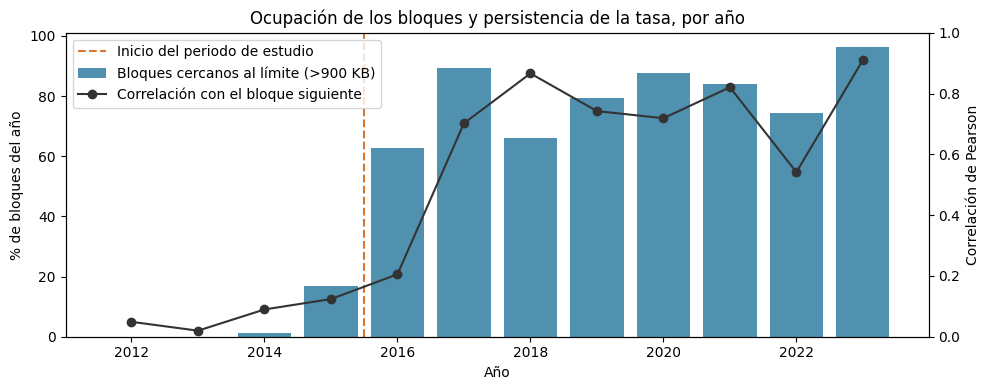
\includegraphics[width=\columnwidth]{ocupacion_por_anio.png}
\caption{Proporción de bloques cercanos al límite de capacidad y correlación de la tasa con la del bloque siguiente, por año.}
\label{fig:ocupacion}
\end{figure}

\subsection{Construcción de la variable objetivo}
La primera formulación usaba un umbral fijo, el percentil 75 de la tasa en entrenamiento (79 sat/byte). Con él, la clase positiva representaba el 24.9\,\% del entrenamiento, pero solo el 0.32\,\% de validación y el 2.4\,\% de prueba, porque el nivel de las comisiones no es estacionario ni siquiera dentro del periodo de estudio: la mediana anual pasa de 134 en 2017 a 8 en 2018 (Fig.~\ref{fig:umbralfijo}). Un umbral constante separa épocas, no bloques caros de baratos dentro de un mismo contexto.

\begin{figure}[htbp]
\centering
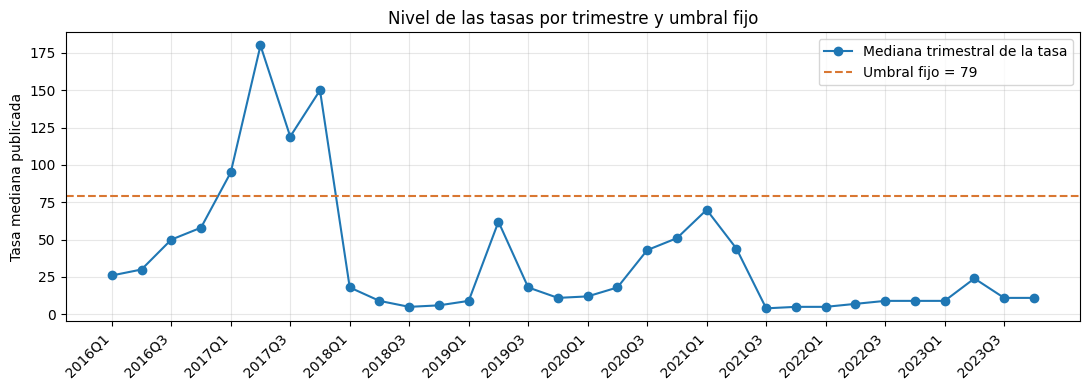
\includegraphics[width=\columnwidth]{nivel_trimestral_umbral_fijo.png}
\caption{Mediana trimestral de la tasa frente al umbral fijo estimado en entrenamiento.}
\label{fig:umbralfijo}
\end{figure}

El umbral móvil de la Ecuación (1) resuelve el problema: la proporción de positivos queda cerca del 25\,\% en las tres particiones (Tabla~\ref{tab:particion}). El resultado es estable para otras ventanas: 24.2/19.4/24.2\,\% con un día y 26.3/22.6/26.0\,\% con un mes. Al descartar las 1007 filas iniciales sin ventana completa quedan 418\,720 ejemplos.

\begin{table}[htbp]
\caption{Partición cronológica}
\label{tab:particion}
\centering
\small
\begin{tabular}{lrlr}
\toprule
Partición & Bloques & Periodo & Positivos \\
\midrule
Entrenamiento & 293\,104 & 2016-01 a 2021-05 & 24.65\,\% \\
Validación & 62\,808 & 2021-05 a 2022-08 & 21.47\,\% \\
Prueba & 62\,808 & 2022-08 a 2023-10 & 24.93\,\% \\
\bottomrule
\end{tabular}
\end{table}

\subsection{Hallazgos relevantes para la predicción}
\textbf{Persistencia del nivel relativo.} Los bloques cuyo sucesor es positivo tienden a presentar ya una tasa por encima de su referencia (Fig.~\ref{fig:transicion}). Cuando el bloque actual supera su umbral, el siguiente lo supera el 52.8\,\% de las veces; cuando no, solo el 15.5\,\%. Esta asimetría sustenta H1 y justifica la persistencia como referencia.

\begin{figure}[htbp]
\centering
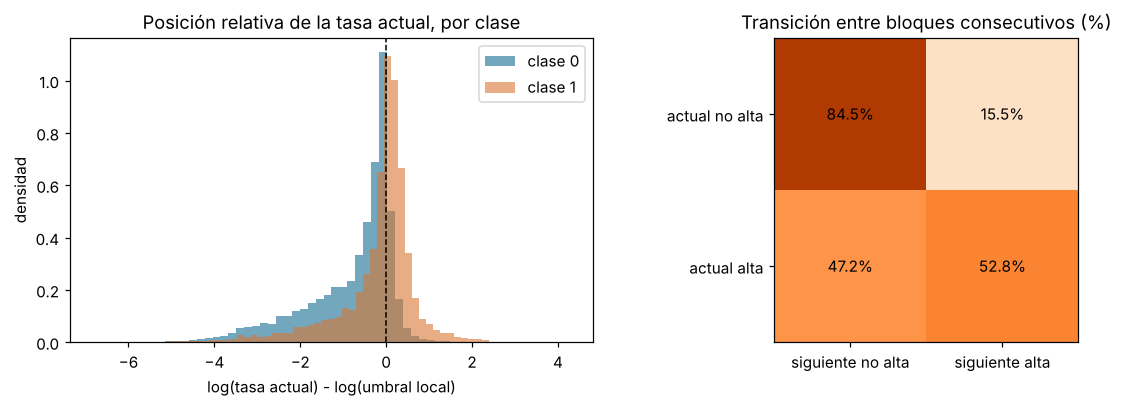
\includegraphics[width=\columnwidth]{eda_posicion_relativa.png}
\caption{Posición relativa de la tasa actual por clase y matriz de transición entre bloques consecutivos (entrenamiento).}
\label{fig:transicion}
\end{figure}

\textbf{Estacionalidad.} La proporción de positivos varía entre 11.3\,\% los domingos y 32.4\,\% los jueves, y entre 15.9\,\% y 37.7\,\% según la hora UTC (Fig.~\ref{fig:calendario}). Parte de este efecto procede de la propia definición de la clase: el umbral promedia una semana completa, de modo que un bloque de domingo se compara con un nivel que incluye la actividad de los días laborables y rara vez lo supera.

\begin{figure}[htbp]
\centering
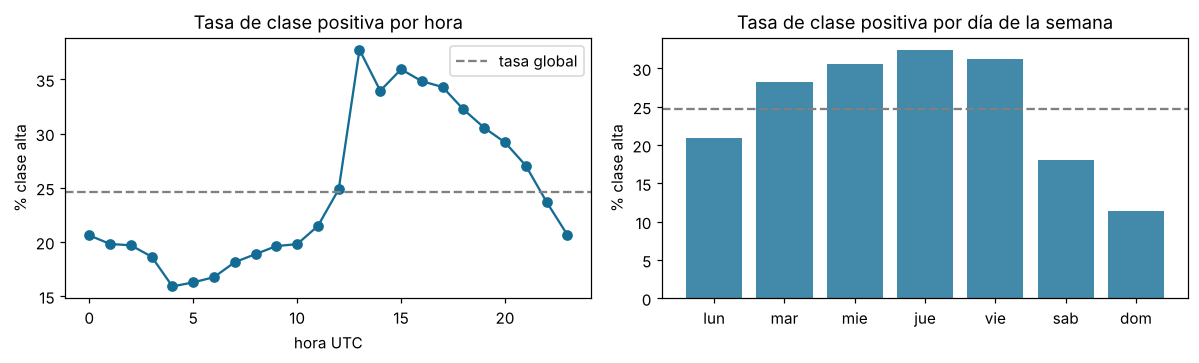
\includegraphics[width=\columnwidth]{eda_calendario.png}
\caption{Proporción de clase positiva por hora UTC y por día de la semana.}
\label{fig:calendario}
\end{figure}

\textbf{Relación entre variables.} La correlación de Spearman con la tasa siguiente es 0.71 para la tasa actual y 0.68 para las comisiones totales, pero solo 0.002 para el tamaño del bloque y 0.11 para el número de transacciones. Una vez que los bloques se llenan de forma habitual, su tamaño deja de informar sobre la congestión. La relación entre la tasa actual y la siguiente es estable entre épocas (Pearson entre 0.76 y 0.90).

\subsection{Prevención de fuga de información}
Se aplican cinco medidas: partición cronológica, nunca aleatoria; umbral calculado solo con bloques hasta $t$; uso de la tasa del bloque siguiente exclusivamente como etiqueta; ajuste de imputadores y escaladores solo con entrenamiento; y margen entre particiones en la validación cruzada. La causalidad de las variables se verificó perturbando bloques futuros y comprobando que las entradas no cambian. En la primera etapa se inspeccionó la proporción de clases en prueba para reformular el objetivo; esa exposición se declara, aunque la prueba no se usó para ajustar ningún modelo.

% =====================================================================
\section{Preprocesamiento e ingeniería de características}
Todas las variables se construyen con información disponible hasta el bloque actual. Se emplearon dos conjuntos, desarrollados de forma independiente por los integrantes del equipo a partir de las propuestas de la primera etapa (Tabla~\ref{tab:features}).

\begin{table}[htbp]
\caption{Conjuntos de variables}
\label{tab:features}
\centering
\small
\setlength{\tabcolsep}{3pt}
\begin{tabular}{p{1.6cm}p{6.4cm}}
\toprule
Grupo & Contenido \\
\midrule
\multicolumn{2}{l}{\textit{Regresión logística (22 variables)}} \\
Nivel relativo & $\log(1+f_t)-\log(1+\theta_t)$, sus rezagos 1, 2, 3 y 6, medias móviles de 6 y 144, volatilidad de 144 y tendencia \\
Dispersión & Razón promedio/mediana y amplitud del rango de tasas \\
Actividad & Ocupación, transacciones relativas, intervalo entre bloques y su media de 6, tamaño medio, entradas y salidas por transacción \\
Calendario & Hora y día en seno y coseno \\
\midrule
\multicolumn{2}{l}{\textit{Modelos de árboles (33 variables)}} \\
Bloque actual & Las 11 columnas numéricas del dataset \\
Comisiones & $\theta_t$, $(f_t+1)/(\theta_t+1)$, razón promedio/mediana, rezagos 1, 6 y 144, medias y desviaciones de 6, 144 y 1008 \\
Actividad & Tamaño, entradas y salidas por transacción, tamaño relativo al máximo de 1008, intervalo entre bloques y bandera de intervalo negativo \\
Calendario & Hora y día en seno y coseno \\
\bottomrule
\end{tabular}
\end{table}

Tres decisiones requieren justificación. Primero, las variables de comisión se expresan \emph{en relación con el umbral local}, porque el nivel absoluto no es estacionario y obligaría al modelo a aprender cortes que dejan de ser válidos al cambiar de periodo; el $+1$ evita divisiones por cero. Segundo, la ocupación se normaliza por el máximo de una ventana móvil y no por el límite nominal de 1~MB, porque la activación de SegWit en 2017 cambió la forma de medir la capacidad. Tercero, los intervalos negativos entre bloques se truncan en cero en la logística y se tratan como faltantes con una bandera explícita en los árboles; en entrenamiento afectan a 1\,491 filas.

Para la regresión logística, la imputación por mediana y la estandarización se ajustan dentro de un \textit{pipeline} solo con entrenamiento, y se descartan las 4\,319 primeras observaciones por el calentamiento de la ventana más larga. Para los árboles se imputa por mediana dentro de cada entrenamiento y no se escalan las variables.

% =====================================================================
\section{Metodología y modelos}
\textbf{Persistencia.} Predice para el bloque siguiente la clase observada en el actual, $\hat y_t = \mathbb{1}[f_t > \theta_t]$. No requiere entrenamiento y es la referencia que cualquier modelo debe superar para aportar sobre la inercia del mercado.

\textbf{Regresión logística regularizada.} Modelo lineal interpretable. Se exploraron penalización L1 y L2, $C \in \{0.01, 0.1, 1, 10\}$ y pesos de clase nulos o balanceados (16 configuraciones), con ajuste posterior del umbral de decisión.

\textbf{Random Forest (RF).} Ensamble de árboles por \textit{bagging} \cite{breiman2001}, capaz de capturar relaciones no lineales e interacciones. Se usaron 100 árboles, \texttt{max\_features=sqrt} y muestras \textit{bootstrap} de la mitad del conjunto de ajuste.

\textbf{HistGradientBoosting (HGB).} Ensamble secuencial por \textit{boosting} \cite{friedman2001} sobre variables discretizadas, eficiente para cientos de miles de ejemplos. Se desactivó la parada temprana interna para evitar una separación aleatoria de los datos.

La Tabla~\ref{tab:busqueda} resume la búsqueda acotada de RF y HGB. Todo se implementó con scikit-learn \cite{sklearn}, con semilla 42.

\begin{table}[htbp]
\caption{Búsqueda de hiperparámetros de los ensambles (F1 medio con umbral 0.5 y AP media en los tres folds temporales)}
\label{tab:busqueda}
\centering
\small
\setlength{\tabcolsep}{3pt}
\begin{tabular}{llcc}
\toprule
Modelo & Configuración & F1 CV & AP CV \\
\midrule
RF & prof. 12, hoja 30 & 0.580 & 0.734 \\
RF & \textbf{prof. 20, hoja 30} & \textbf{0.589} & 0.738 \\
RF & sin límite, hoja 80 & 0.581 & 0.733 \\
HGB & 120 it., 15 hojas, $\eta$=0.08, L2=1 & 0.619 & 0.743 \\
HGB & 180 it., 31 hojas, $\eta$=0.06, L2=5 & 0.627 & 0.748 \\
HGB & \textbf{180 it., 15 hojas, $\eta$=0.10, L2=5} & \textbf{0.630} & 0.747 \\
\bottomrule
\end{tabular}
\end{table}

En la regresión logística, las 16 configuraciones quedaron dentro de 0.0003 de F1 tras ajustar el umbral; se eligió L2, $C=1$, sin ponderación. Con 288\,784 observaciones y 22 variables no hay margen de sobreajuste que la penalización deba corregir. El ajuste del umbral influyó mucho más que la regularización: con el corte de 0.5 el F1 era 0.417, y con el umbral ajustado (0.312) subió a 0.558.

% =====================================================================
\section{Diseño experimental y evaluación}
\textbf{Ensambles.} La selección usó tres folds de ventana expansiva dentro de entrenamiento, con 40\,000 ejemplos de validación interna y un margen de 1008 bloques entre ajuste y validación (Tabla~\ref{tab:folds}). Se eligió por familia el candidato de mayor F1 medio y, después, el umbral de probabilidad que maximiza el F1 de sus predicciones fuera de fold, en una malla de 0.10 a 0.90 con paso 0.025. Los modelos elegidos se reajustaron con las primeras 292\,096 filas de entrenamiento, reservando las últimas 1008 como margen, y se evaluaron una sola vez en validación.

\begin{table}[htbp]
\caption{Folds de validación cruzada temporal (ventana expansiva, \textit{gap} de 1008 bloques)}
\label{tab:folds}
\centering
\small
\begin{tabular}{clll}
\toprule
Fold & Ajuste & Validación interna & Positivos \\
\midrule
1 & 2016-01 a 2019-02 & 2019-03 a 2019-11 & 25.2\,\% \\
2 & 2016-01 a 2019-11 & 2019-11 a 2020-08 & 26.2\,\% \\
3 & 2016-01 a 2020-08 & 2020-08 a 2021-05 & 26.6\,\% \\
\bottomrule
\end{tabular}
\end{table}

\textbf{Regresión logística.} La configuración y el umbral se seleccionaron directamente sobre validación, por lo que su F1 de validación es optimista frente al de los ensambles. La prueba se evaluó una sola vez, después de fijar todas las decisiones.

\textbf{Métricas.} El F1 de la clase alta es la métrica principal. La AP resume la curva precisión--exhaustividad sin depender del umbral y es más informativa que el ROC-AUC con clases desbalanceadas. Para comparar conjuntos de variables se usó un \textit{bootstrap} emparejado por bloques móviles de 1008 bloques \cite{kunsch1989}, con 1000 remuestreos, que conserva la dependencia entre bloques consecutivos.

% =====================================================================
\section{Resultados}
\subsection{Comparación de métodos}
Para la evaluación final de RF y HGB se conservaron los ajustes originales sobre 292\,096 filas de entrenamiento, sin reajustar con validación, y los umbrales OOF de 0.300 y 0.350. Se reprodujeron las probabilidades de validación de ambas familias antes de evaluar los 62\,808 ejemplos de prueba. No se realizaron búsquedas ni ajustes del umbral en prueba.

La Tabla~\ref{tab:resultados} reúne los cuatro métodos. En validación, RF y HGB superan a la persistencia en F1 (+0.024 y +0.032) y a la regresión logística en AP (+0.030 y +0.037). En prueba, la persistencia supera a la regresión logística en F1 (0.5763 frente a 0.5704), aunque esta discrimina claramente mejor que el azar: su AP es 0.617, 2.5 veces la tasa base de 0.249 (Fig.~\ref{fig:logistica}).

En prueba, RF y HGB superan a la persistencia en F1 por 0.0285 y 0.0330, respectivamente. Sus AP son 0.6838 y 0.6898, frente a 0.6166 de la logística. Estas diferencias son descriptivas y no demuestran significancia estadística; además, la logística y los árboles emplean conjuntos de variables diferentes.

\begin{table}[htbp]
\caption{Resultados de los cuatro métodos. La persistencia solo emite etiquetas, por lo que no tiene AP ni ROC-AUC.}
\label{tab:resultados}
\centering
\small
\setlength{\tabcolsep}{4pt}
\begin{tabular}{llccccc}
\toprule
Método & Part. & F1 & Prec. & Rec. & AP & ROC \\
\midrule
Persistencia & Val. & 0.5398 & 0.5405 & 0.5391 & -- & -- \\
Logística & Val. & 0.5572 & 0.5157 & 0.6060 & 0.5929 & 0.8090 \\
RF & Val. & 0.5638 & 0.5966 & 0.5344 & 0.6225 & 0.8171 \\
HGB & Val. & 0.5713 & 0.5608 & 0.5823 & 0.6298 & 0.8217 \\
\midrule
Persistencia & Prueba & 0.5763 & 0.5770 & 0.5755 & -- & -- \\
Logística & Prueba & 0.5704 & 0.5478 & 0.5950 & 0.6166 & 0.8061 \\
RF & Prueba & 0.6048 & 0.5947 & 0.6152 & 0.6838 & 0.8283 \\
HGB & Prueba & 0.6093 & 0.5704 & 0.6538 & 0.6898 & 0.8328 \\
\bottomrule
\end{tabular}
\end{table}

\begin{figure*}[t]
\centering
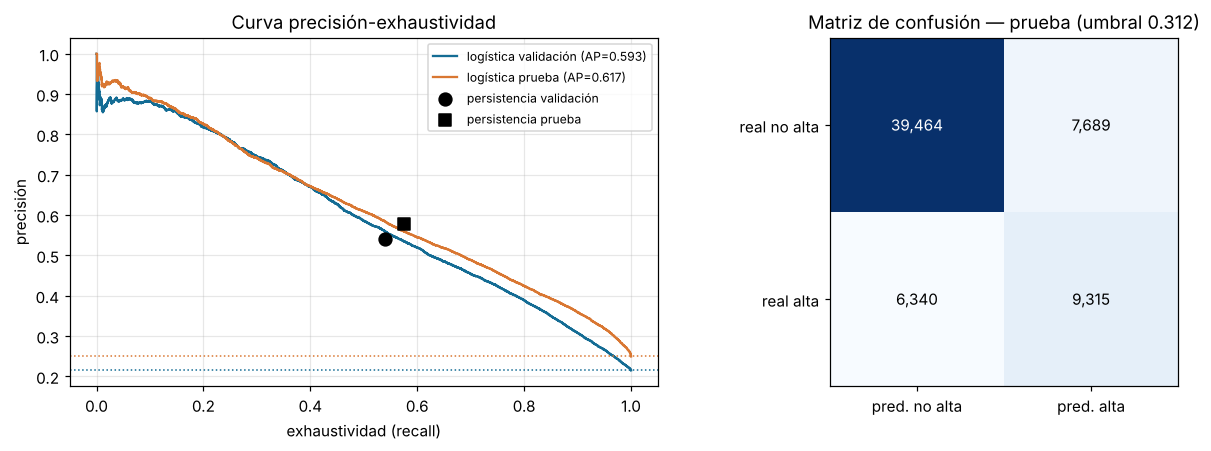
\includegraphics[width=0.75\textwidth]{pr_y_matriz_confusion.png}
\caption{Regresión logística: curvas precisión--exhaustividad en validación y prueba, con el punto de operación de la persistencia, y matriz de confusión en prueba (umbral 0.312).}
\label{fig:logistica}
\end{figure*}

El resultado de la logística no se explica por la transferencia del umbral: el umbral óptimo en prueba sería 0.271 en lugar de 0.312, y la diferencia cuesta 0.007 de F1. Incluso con ese umbral, calculado solo como diagnóstico, el modelo alcanzaría 0.5776 frente a 0.5763 de la persistencia. En prueba produce 9\,315 verdaderos positivos, 7\,689 falsos positivos y 6\,340 falsos negativos.

\begin{figure}[htbp]
\centering
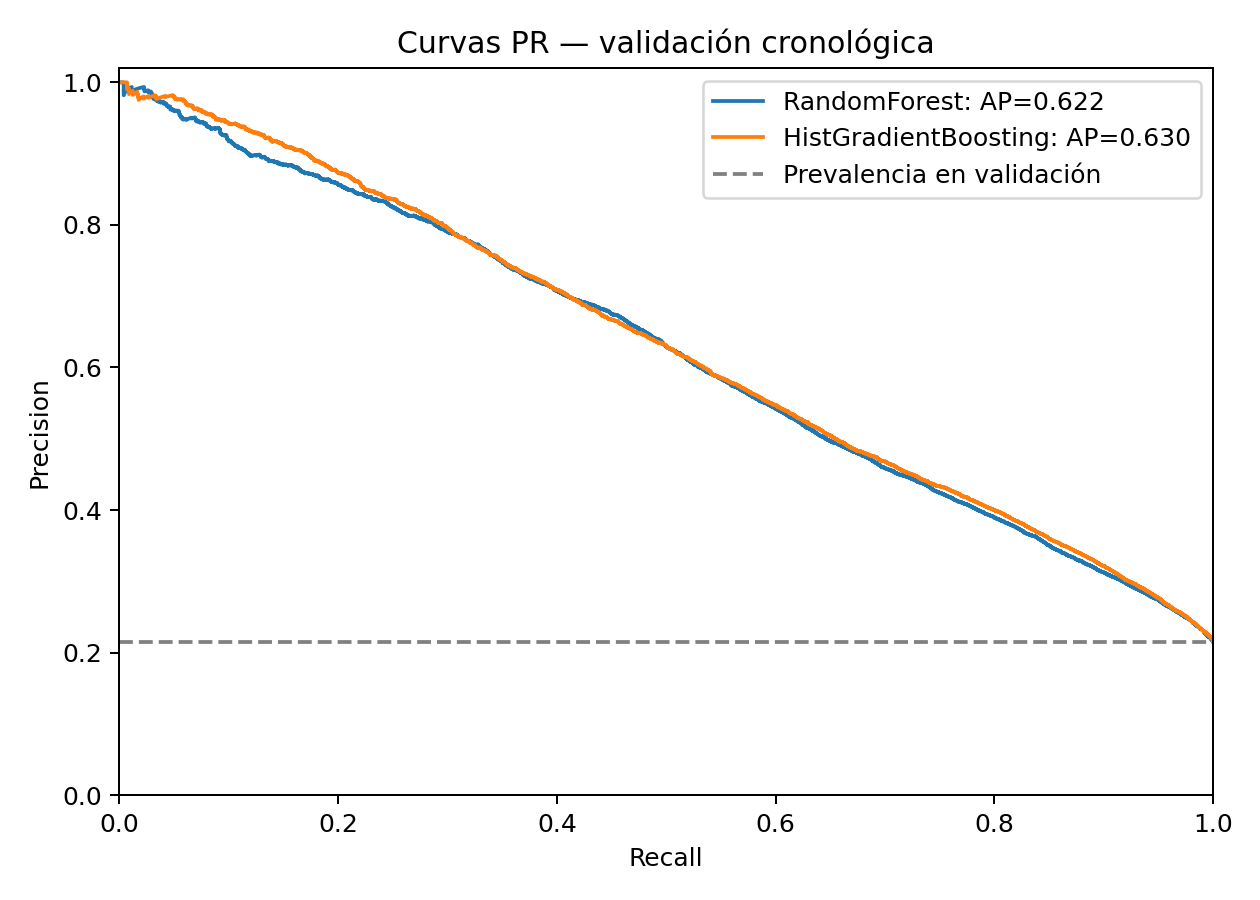
\includegraphics[width=0.9\columnwidth]{curvas_pr.png}
\caption{Curvas precisión--exhaustividad de RF y HGB en validación.}
\label{fig:pr}
\end{figure}

Las curvas de RF y HGB (Fig.~\ref{fig:pr}) se mantienen por encima de la prevalencia en todo el rango. Con los umbrales fijados en los folds (0.300 para RF y 0.350 para HGB), RF produce 7\,208 verdaderos positivos y 4\,873 falsos positivos, y HGB 7\,853 y 6\,150 (Fig.~\ref{fig:matrices}): HGB detecta 645 positivos más a cambio de 1\,277 falsos positivos adicionales.

\begin{figure}[htbp]
\centering
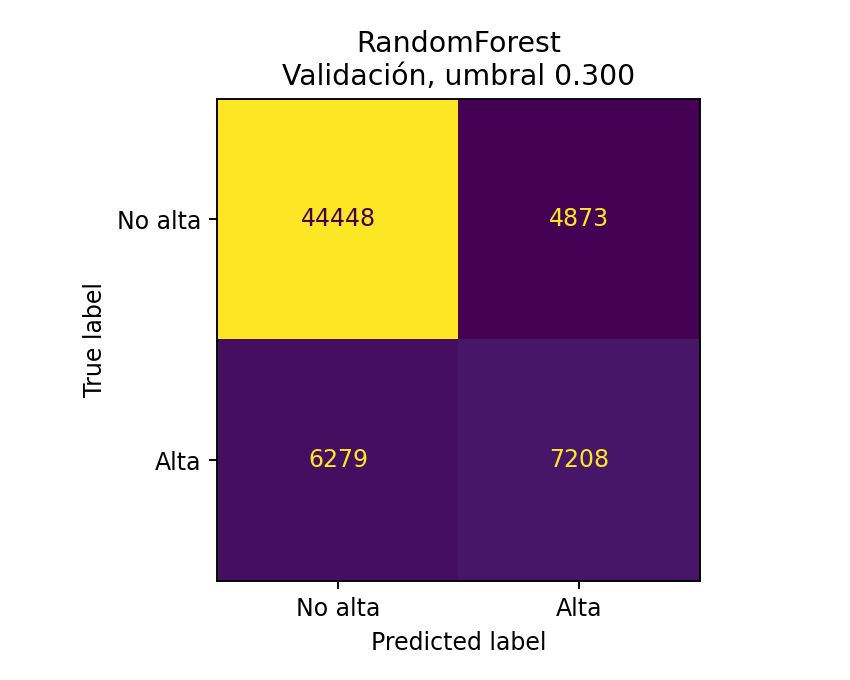
\includegraphics[width=0.49\columnwidth]{matriz_RandomForest.png}\hfill
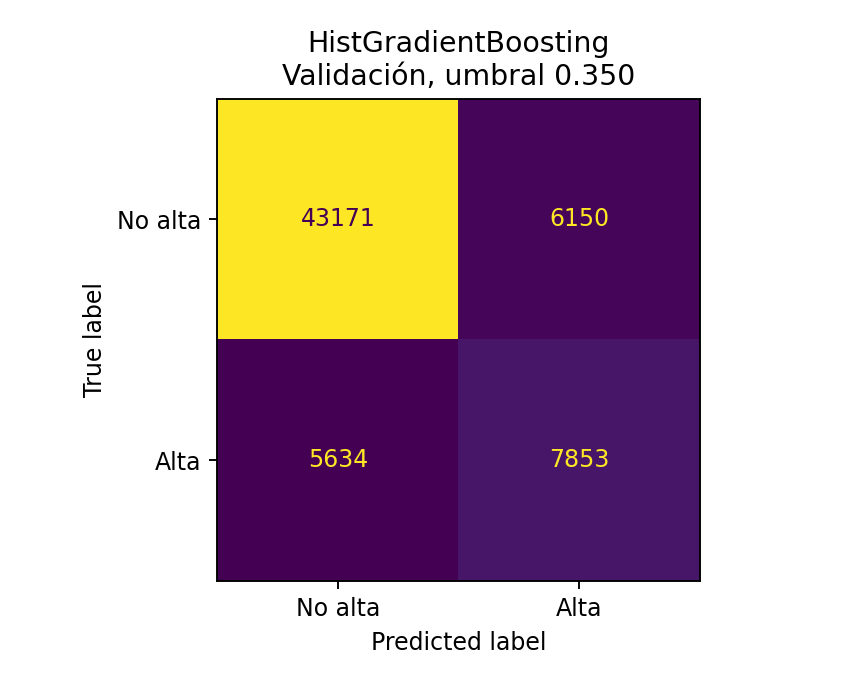
\includegraphics[width=0.49\columnwidth]{matriz_HistGradientBoosting.png}
\caption{Matrices de confusión de RF y HGB en validación.}
\label{fig:matrices}
\end{figure}

\textbf{Generalización.} El F1 sobre los datos de ajuste es 0.632 para RF y 0.582 para HGB, frente a 0.564 y 0.571 en validación (Fig.~\ref{fig:brecha}). La brecha mayor de RF sugiere más sobreajuste, aunque parte de la diferencia también puede deberse al cambio temporal entre periodos.

\begin{figure}[htbp]
\centering
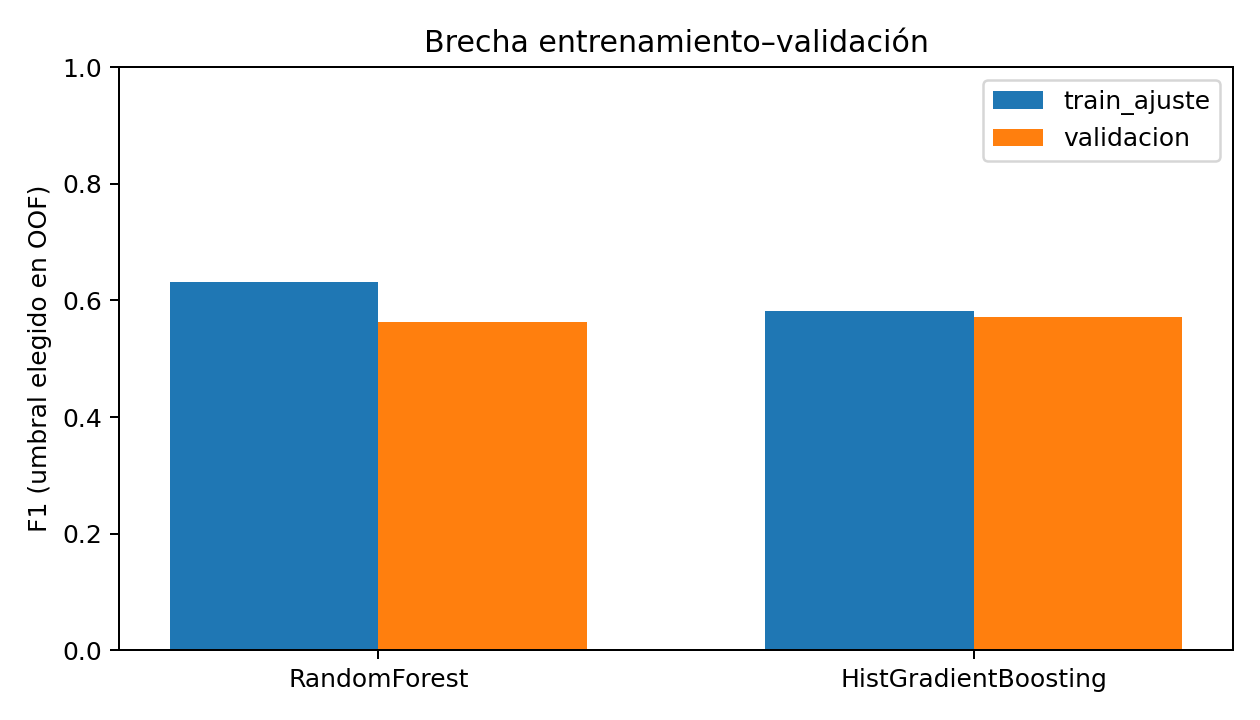
\includegraphics[width=0.85\columnwidth]{brecha_generalizacion.png}
\caption{F1 en los datos de ajuste y en validación.}
\label{fig:brecha}
\end{figure}

\textbf{Interpretación de variables.} La importancia por reducción de impureza de RF está dominada por la tasa relativa al umbral (0.31), seguida por las medias móviles de la tasa de 6 y 1008 bloques; las variables de volumen quedan por debajo de 0.02 (Fig.~\ref{fig:importancia}). En la regresión logística, los mayores coeficientes corresponden a las medias móviles de 144 y 6 bloques (0.81 y 0.49) y a la volatilidad reciente (0.43), seguidos por la hora del día ($-$0.33) (Fig.~\ref{fig:coeficientes}). Ambas medidas son descriptivas y están afectadas por la correlación entre variables.

\begin{figure}[htbp]
\centering
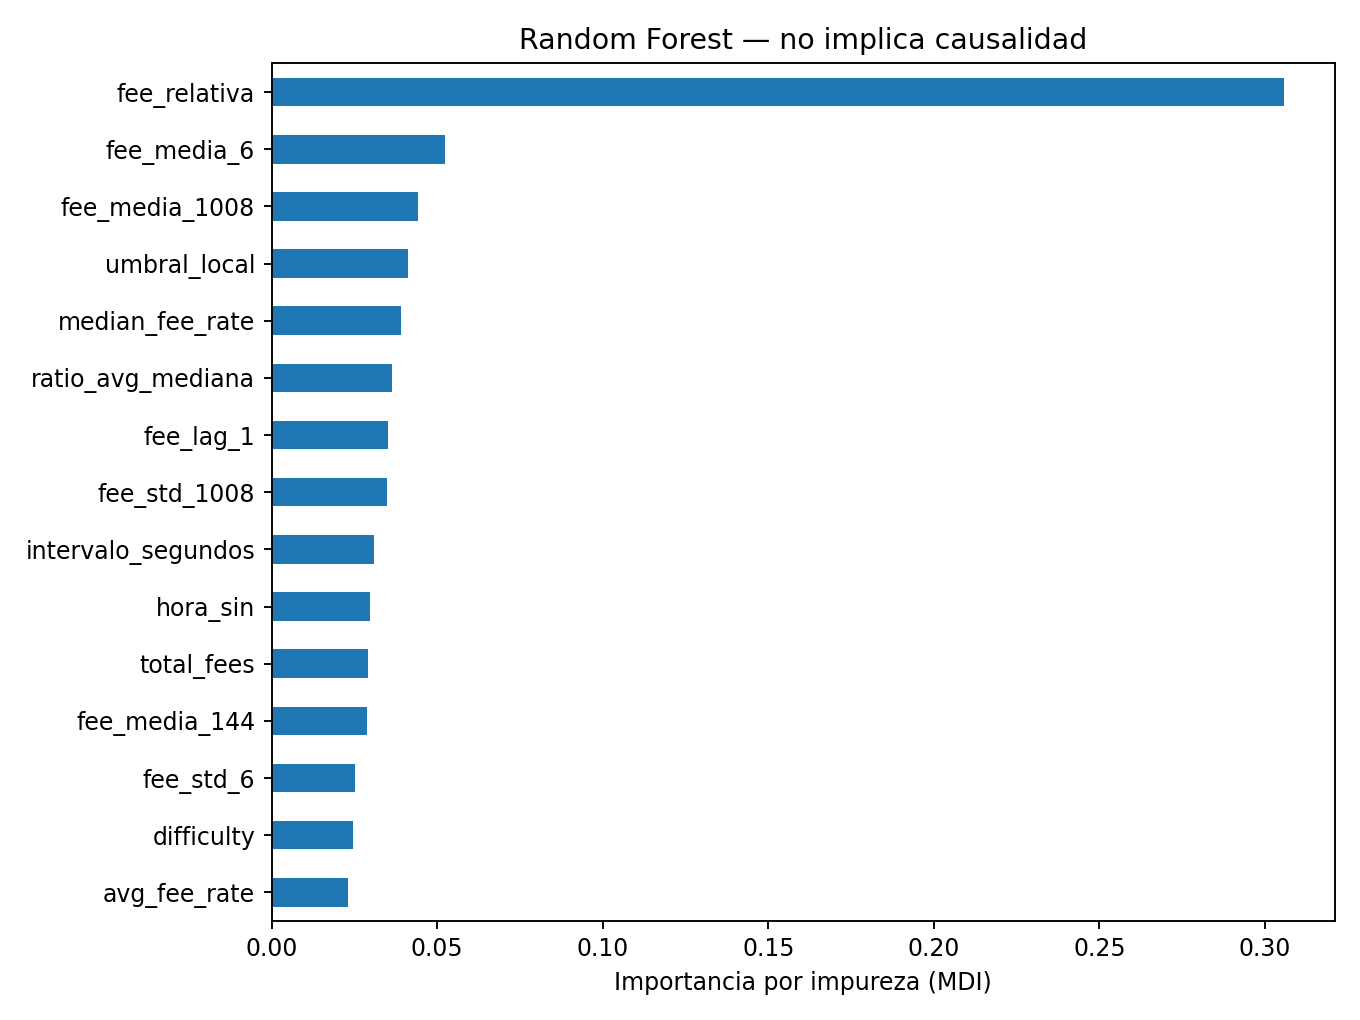
\includegraphics[width=0.9\columnwidth]{importancia_rf_mdi.png}
\caption{Importancia por reducción de impureza de las 15 variables principales de RF.}
\label{fig:importancia}
\end{figure}

\begin{figure}[htbp]
\centering
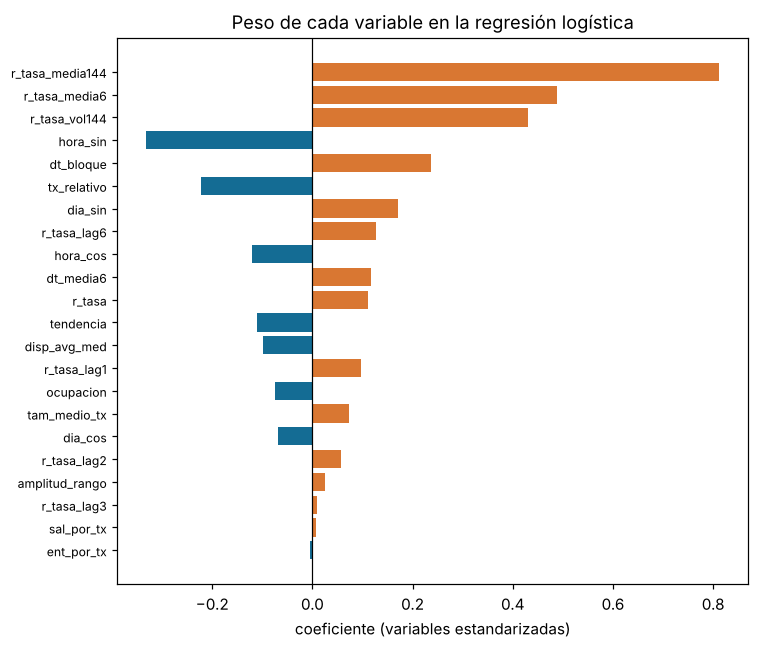
\includegraphics[width=0.8\columnwidth]{coeficientes_logistica.png}
\caption{Coeficientes de la regresión logística con variables estandarizadas.}
\label{fig:coeficientes}
\end{figure}

\subsection{Estudio de ablación}
Para aislar el aporte de cada grupo de variables se entrenó un mismo HGB, con la configuración ganadora de la búsqueda (180 iteraciones, 15 hojas, tasa 0.1, hoja mínima 80, L2 de 5), con cuatro subconjuntos de las 33 variables, usando los mismos folds, margen y criterio de umbral: A0, la tasa actual ($f_t$, $\theta_t$ y su razón; 3 variables); A, todas las de comisiones (16); B, comisiones y actividad de la red, incluidas las comisiones totales como se planteó en H2 (29); y C, todas (33). Como control, el conjunto C reproduce exactamente el HGB de la Tabla~\ref{tab:resultados} (F1 de 0.571 y AP de 0.630 en validación). Los resultados se muestran en la Tabla~\ref{tab:ablation} y la Fig.~\ref{fig:ablation}.

\begin{table}[htbp]
\caption{Ablación en validación. $\Delta$AP frente al conjunto anterior, con IC 95\,\% por \textit{bootstrap} de bloques.}
\label{tab:ablation}
\centering
\small
\setlength{\tabcolsep}{3.5pt}
\begin{tabular}{lcccc}
\toprule
Conjunto & Var. & AP & F1 & $\Delta$AP [IC 95\,\%] \\
\midrule
A0: tasa actual & 3 & 0.535 & 0.539 & -- \\
A: comisiones & 16 & 0.622 & 0.569 & +0.088 [0.075, 0.099] \\
B: + actividad & 29 & 0.629 & 0.565 & +0.007 [0.003, 0.011] \\
C: + calendario & 33 & 0.630 & 0.571 & +0.001 [$-$0.005, 0.005] \\
Persistencia & -- & -- & 0.540 & -- \\
\bottomrule
\end{tabular}
\end{table}

\begin{figure}[htbp]
\centering
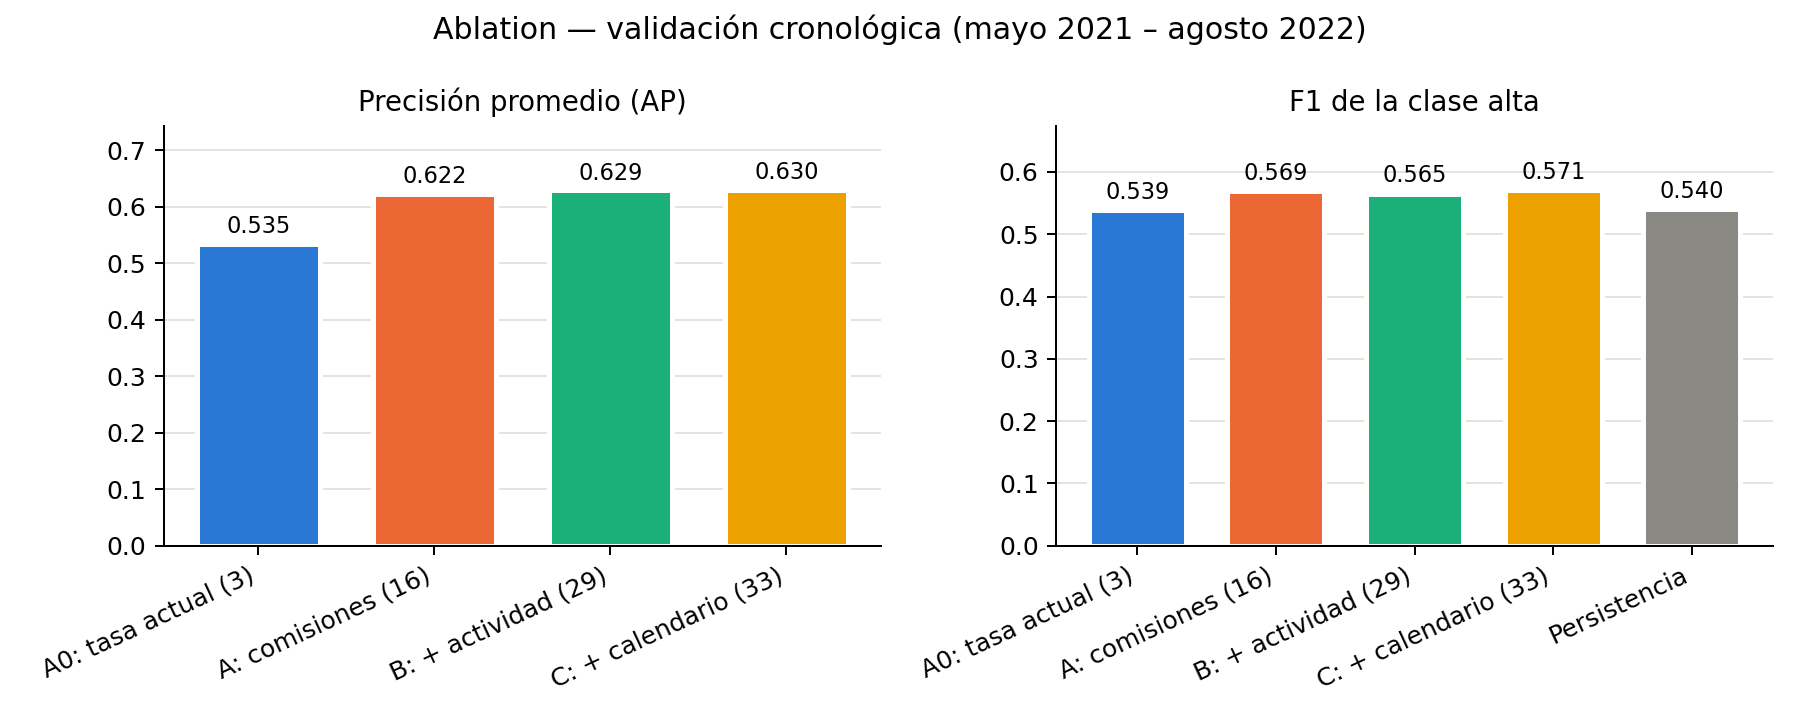
\includegraphics[width=\columnwidth]{ablation_validacion.png}
\caption{Ablación: AP y F1 en validación por conjunto de variables.}
\label{fig:ablation}
\end{figure}

Con solo la tasa actual, el modelo obtiene el mismo F1 que la persistencia (0.539 frente a 0.540): con tres variables, aprende la misma regla. La historia de las comisiones aporta la mayor mejora (+0.030 de F1, IC [0.023, 0.038]). La actividad de la red añade una mejora pequeña pero detectable en AP, y el calendario no cambia la AP. En F1, las diferencias entre A, B y C son pequeñas y de signo variable (B frente a A: $-$0.004, IC [$-$0.009, 0.001]; C frente a B: +0.006, IC [0.000, 0.012]), porque dependen del umbral elegido en cada caso (0.275 para A y 0.350 para B y C); por eso la comparación se basa en la AP. El mismo orden (A0 $<$ A $<$ B $\approx$ C en AP) se observa en los tres folds de entrenamiento, con AP de 0.59--0.70 para A0 y de 0.69--0.79 para B.

\subsection{Rendimiento por periodos y volatilidad}
Por trimestre de validación, el F1 varía entre 0.50 y 0.64 de forma paralela en todos los métodos y sigue la proporción de positivos: los trimestres con menos bloques altos (2021T3 y 2022T1, alrededor del 19\,\%) son los de menor F1 (Fig.~\ref{fig:trimestre}). La ventaja de los modelos con historia de comisiones sobre la persistencia es positiva en todos los trimestres (+0.02 a +0.04 para el conjunto C).

\begin{figure}[htbp]
\centering
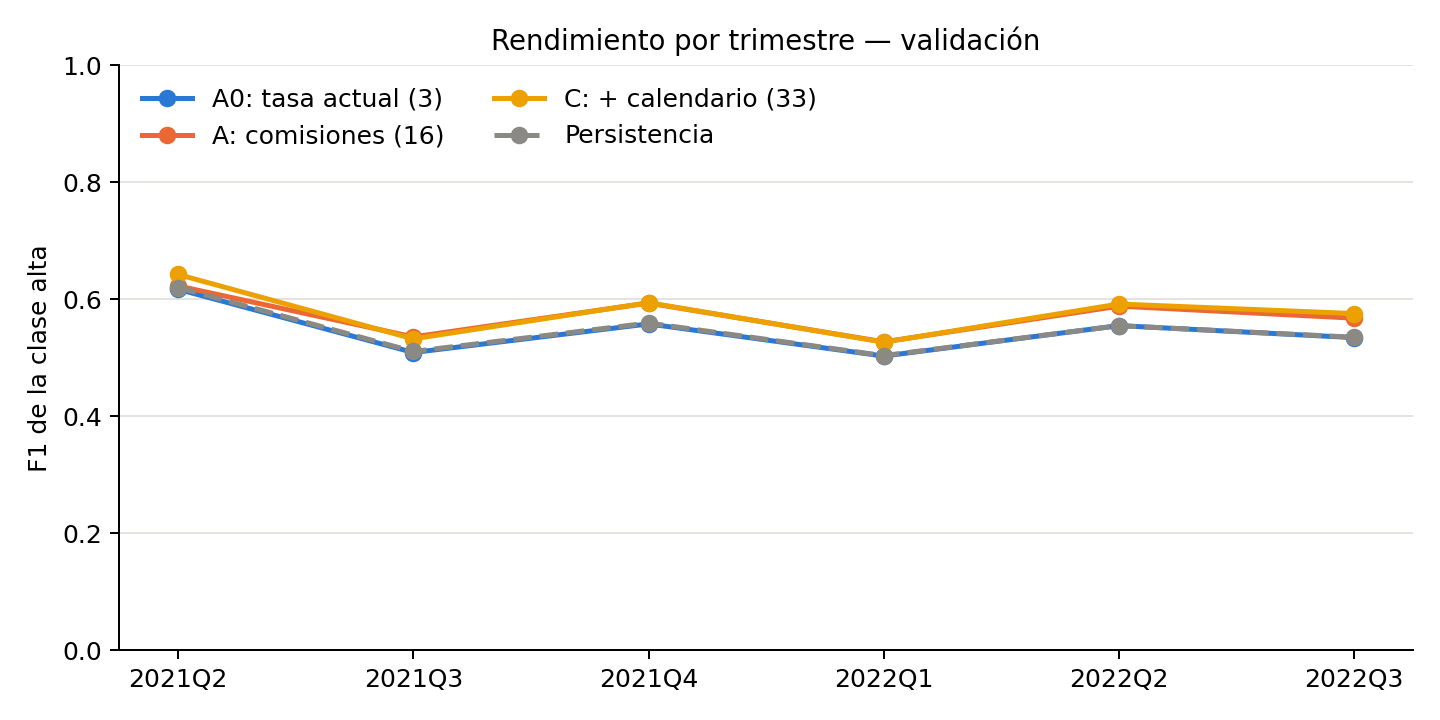
\includegraphics[width=\columnwidth]{f1_por_trimestre.png}
\caption{F1 por trimestre de validación.}
\label{fig:trimestre}
\end{figure}

La volatilidad reciente se midió con el coeficiente de variación de las últimas 144 tasas, con terciles fijados en entrenamiento. El F1 del modelo con las 33 variables es 0.567, 0.582 y 0.554 en volatilidad baja, media y alta, y su AP 0.626, 0.643 y 0.596 (Fig.~\ref{fig:volatilidad}). En el tercil alto hay menos positivos (16\,\% frente a 21--23\,\%), lo que reduce el F1 de forma mecánica, y solo el 11\,\% de los bloques de validación cae en ese tercil.

\begin{figure}[htbp]
\centering
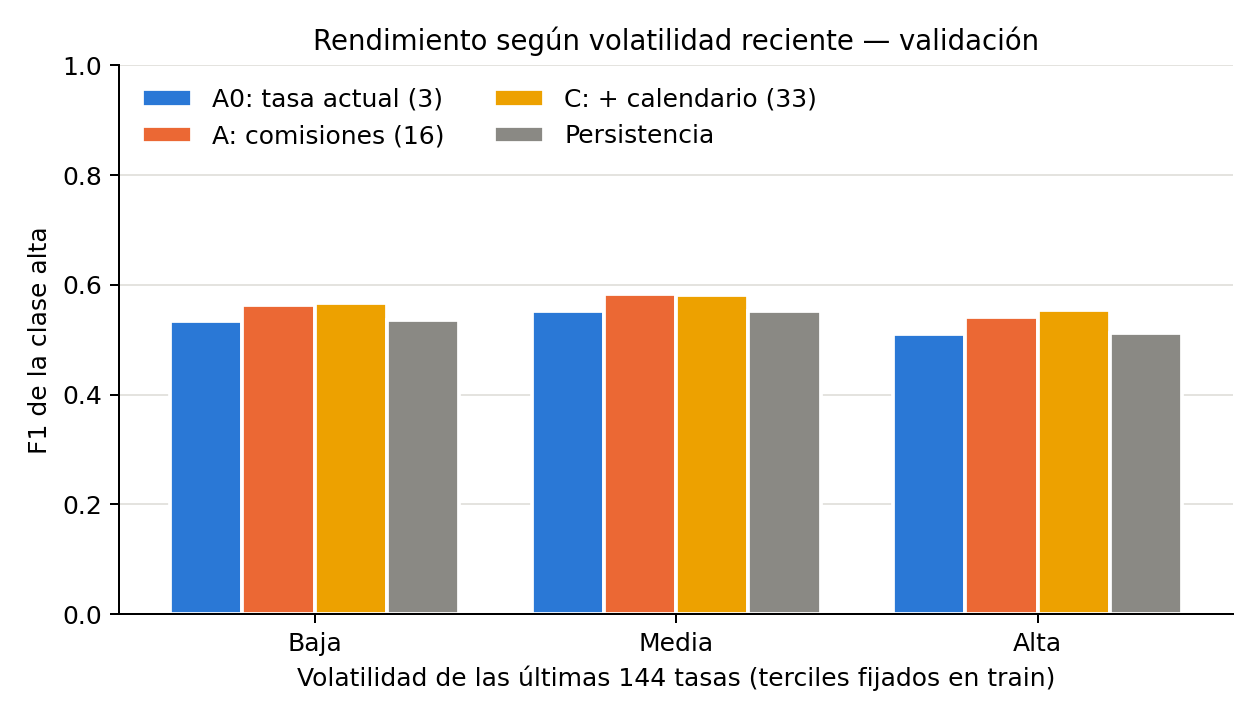
\includegraphics[width=0.9\columnwidth]{f1_por_volatilidad.png}
\caption{F1 según la volatilidad reciente en validación.}
\label{fig:volatilidad}
\end{figure}

\subsection{Análisis de errores}
El 19.8\,\% de los bloques de validación es un cambio de clase, y un episodio de comisión alta dura en promedio 2.17 bloques, poco más de veinte minutos. La persistencia falla, por construcción, en todas esas transiciones y acierta en todos los tramos estables. El modelo con las 33 variables anticipa el 35\,\% de los finales de episodio, pero solo el 19\,\% de los inicios, a cambio de errar en el 4.9\,\% de los tramos bajos estables y en el 8.5\,\% de los altos (Fig.~\ref{fig:transiciones}).

\begin{figure}[htbp]
\centering
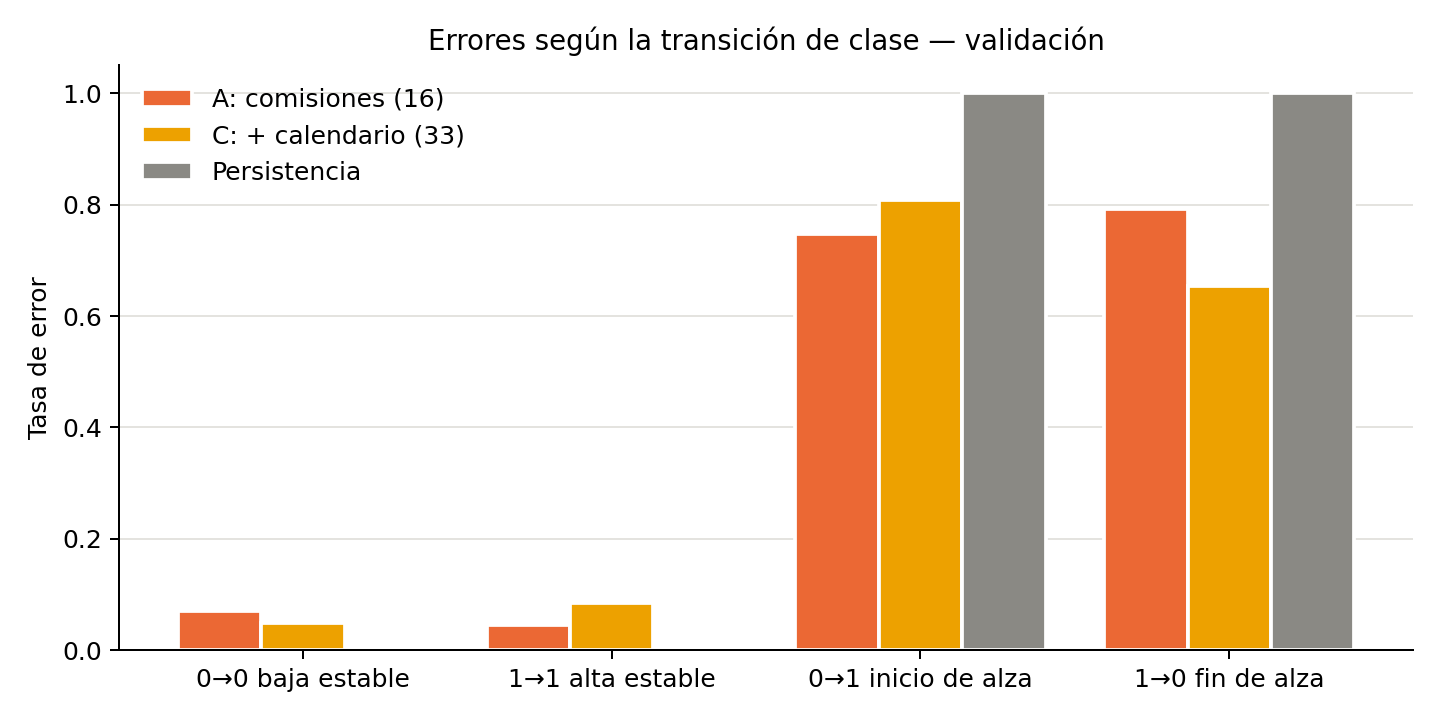
\includegraphics[width=\columnwidth]{errores_por_transicion.png}
\caption{Tasa de error según la transición de clase en validación.}
\label{fig:transiciones}
\end{figure}

Los errores se concentran cerca del umbral (Fig.~\ref{fig:margen}). La tasa de error es del 8\,\% cuando la tasa del bloque siguiente queda por debajo de la mitad del umbral y del 72\,\% cuando lo supera por menos del 5\,\%. Los falsos positivos son bloques actuales caros (razón mediana con el umbral de 1.14) seguidos de uno algo más barato (margen mediano 0.79); los falsos negativos, bloques baratos (0.69) seguidos de uno que supera el umbral (1.25). La volatilidad reciente es casi igual en los cuatro tipos de predicción, y los errores se agrupan en el tiempo: la probabilidad de error tras un error es 0.42, frente a 0.19 en general.

\begin{figure}[htbp]
\centering
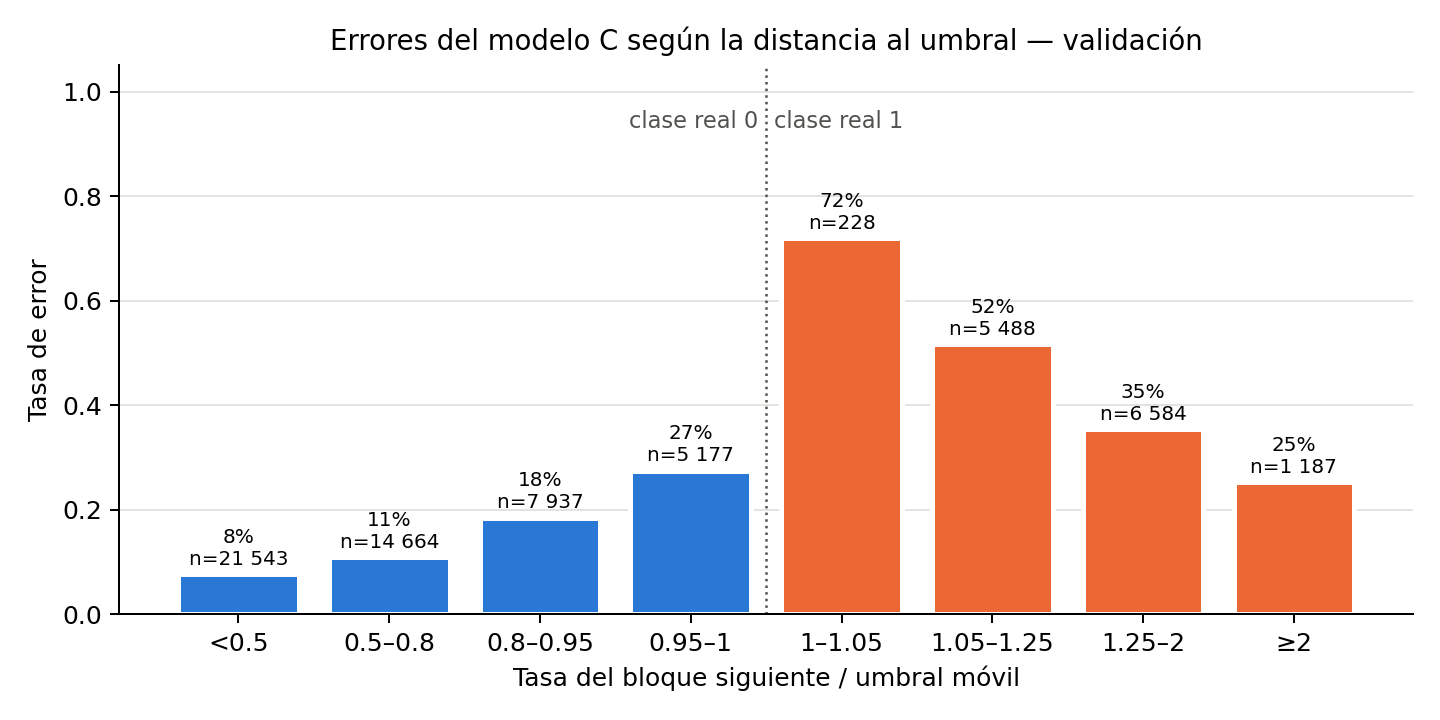
\includegraphics[width=\columnwidth]{errores_por_margen.png}
\caption{Tasa de error según la razón entre la tasa del bloque siguiente y el umbral móvil.}
\label{fig:margen}
\end{figure}

% =====================================================================
\section{Discusión}
\textbf{Origen de la capacidad predictiva.} La información útil procede de la historia reciente de las comisiones y no del estado instantáneo de la red. El estado actual equivale a la persistencia; la mejora aparece al describir la tendencia y la inestabilidad recientes del precio. Esta lectura coincide en los tres enfoques: el ablation, la importancia de RF y los coeficientes de la logística, donde dominan las medias móviles y la volatilidad.

\textbf{Por qué los árboles superan a la logística.} Con variables de contenido similar, los árboles obtienen una AP mayor. Esto sugiere que la relación entre la historia de la tasa y la clase siguiente no es lineal: el efecto de una variable, como la volatilidad reciente, puede depender de qué tan cerca esté la tasa actual del umbral, una interacción que los árboles representan de forma natural. La logística, cuyas 16 configuraciones rinden igual, parece limitada por su forma funcional y no por la regularización. Entre los ensambles, HGB generaliza algo mejor que RF, con una brecha menor entre ajuste y validación.

\textbf{Actividad de la red y calendario.} La actividad aporta poco porque, desde 2016, los bloques están casi siempre llenos: su tamaño y su número de transacciones varían poco, y la congestión se manifiesta en el precio y no en el volumen. El calendario muestra señal en la logística, pero no añade nada a los árboles una vez incluidas las medias móviles de 6 y 144 bloques, que ya recogen el ciclo diario. Además, parte de esa señal procede de la propia ventana semanal del umbral, por lo que no debe interpretarse como una propiedad del mercado.

\textbf{Techo de rendimiento.} La ventaja sobre la persistencia es consistente pero modesta en F1. Los episodios de comisión alta son muy cortos, y su inicio corresponde a la llegada de demanda nueva que todavía no se refleja en los bloques minados. Además, muchas etiquetas dependen de diferencias de uno o dos satoshis por byte respecto a un umbral que se mueve en cada bloque. Ambas condiciones limitan el rendimiento alcanzable con estas variables, independientemente del algoritmo. La diferencia en AP es mayor que en F1: los modelos ordenan bien los bloques según su riesgo, aunque un único umbral binario recorte parte de esa ventaja.

\subsection{Limitaciones}
\begin{itemize}
\item \textbf{Ausencia del \textit{mempool}.} La demanda pendiente, que anticipa la congestión, no es observable; limita sobre todo la detección del inicio de los episodios.
\item \textbf{Datos agregados y sesgo de selección.} Cada observación resume un bloque y solo incluye transacciones confirmadas.
\item \textbf{Frontera de la clase.} Muchas etiquetas quedan muy cerca del umbral, y las inconsistencias de la fuente pueden alterar la clase asignada.
\item \textbf{Dependencia temporal.} Los intervalos de \textit{bootstrap} son aproximados y no se corrigen por comparaciones múltiples.
\item \textbf{Conjuntos de variables distintos.} La logística (22 variables) y los árboles (33) no comparten exactamente las mismas entradas, por lo que su comparación mezcla el efecto del algoritmo y el de las variables.
\item \textbf{Selección del umbral de la logística en validación,} cuya proporción de positivos (21.5\,\%) difiere de la de prueba (24.9\,\%).
\item \textbf{Validación tranquila,} con pocos episodios de alta volatilidad.
\item \textbf{Alcance del ablation,} obtenido con un solo algoritmo y la configuración elegida con las 33 variables, sin reajustarla para cada subconjunto.
\item \textbf{Periodo de estudio,} limitado a 2016--2023.
\end{itemize}

\subsection{Consideraciones éticas}
El modelo describe el mercado agregado y no utiliza información personal. Sin embargo, un uso operativo podría llevar a los usuarios a retrasar o adelantar transacciones con base en una predicción que falla con frecuencia justo al inicio de la congestión, cuando equivocarse cuesta más. Cualquier aplicación debería comunicar esa incertidumbre y no presentarse como un estimador completo de comisiones. Los resultados tampoco deberían generalizarse a otras redes o periodos sin una nueva validación.

% =====================================================================
\section{Conclusiones}
Este trabajo evaluó si las estadísticas históricas a nivel de bloque permiten anticipar si el siguiente bloque de Bitcoin tendrá comisiones elevadas respecto a la semana anterior.

\begin{itemize}
\item \textbf{H1 se confirma:} la tasa reciente es el predictor dominante. Sin embargo, el estado actual por sí solo equivale a la persistencia; el valor aparece al incorporar la historia reciente de las comisiones (+0.088 de AP).
\item \textbf{H2 se confirma:} la actividad de la red aporta una mejora pequeña pero detectable (+0.007 de AP), muy inferior a la de la historia de comisiones, y el calendario no aporta información adicional.
\item \textbf{H3 se confirma parcialmente:} el rendimiento disminuye en el tercil de mayor volatilidad de forma moderada. La principal fuente de error son los cambios de clase, sobre todo el inicio de los episodios de comisión alta.
\end{itemize}

La persistencia es una referencia difícil de superar: la regresión logística no lo logra en prueba, mientras que RF y HGB sí la superan, con F1 de 0.6048 y 0.6093 frente a 0.5763. La ventaja descriptiva de los árboles se observa tanto en validación como en prueba; no se ha establecido su significancia estadística. El aprendizaje principal es que el límite no está en el algoritmo, sino en la información disponible: sin el estado del \textit{mempool}, la llegada de nueva demanda no puede anticiparse.

Como trabajo futuro se propone incorporar datos del \textit{mempool} o de tasas ofrecidas en tiempo real; plantear la detección del inicio de los episodios de congestión como una tarea propia; evaluar horizontes de predicción mayores que un bloque; unificar el conjunto de variables entre modelos; y definir la clase con un margen alrededor del umbral que reduzca la ambigüedad de las etiquetas.

\section*{Repositorio}
El código, los notebooks y los resultados están disponibles en \url{https://github.com/naye-gg/bitcoin-block-fee-classification_ML_project} \cite{repo}.

\begin{thebibliography}{00}
\bibitem{moser2015} M. Möser and R. Böhme, ``Trends, tips, tolls: A longitudinal study of Bitcoin transaction fees,'' in \textit{Financial Cryptography and Data Security}, LNCS 8976, Springer, 2015, pp. 19--33.
\bibitem{easley2019} D. Easley, M. O'Hara, and S. Basu, ``From mining to markets: The evolution of Bitcoin transaction fees,'' \textit{J. Financial Economics}, vol. 134, no. 1, pp. 91--109, 2019.
\bibitem{huberman2021} G. Huberman, J. D. Leshno, and C. Moallemi, ``Monopoly without a monopolist: An economic analysis of the Bitcoin payment system,'' \textit{Rev. Economic Studies}, vol. 88, no. 6, pp. 3011--3040, 2021.
\bibitem{graterol_kaggle} J. Graterol, ``Bitcoin Blockchain Historical Data,'' Kaggle. [Online]. Available: \url{https://www.kaggle.com/datasets/jesusgraterol/bitcoin-blockchain-dataset}
\bibitem{graterol_github} J. Graterol, ``Bitcoin Blockchain Dataset Builder,'' GitHub. [Online]. Available: \url{https://github.com/jesusgraterol/bitcoin-blockchain-dataset-builder}
\bibitem{breiman2001} L. Breiman, ``Random forests,'' \textit{Machine Learning}, vol. 45, no. 1, pp. 5--32, 2001.
\bibitem{friedman2001} J. H. Friedman, ``Greedy function approximation: A gradient boosting machine,'' \textit{Ann. Statist.}, vol. 29, no. 5, pp. 1189--1232, 2001.
\bibitem{sklearn} F. Pedregosa \textit{et al.}, ``Scikit-learn: Machine learning in Python,'' \textit{J. Mach. Learn. Res.}, vol. 12, pp. 2825--2830, 2011.
\bibitem{kunsch1989} H. R. Künsch, ``The jackknife and the bootstrap for general stationary observations,'' \textit{Ann. Statist.}, vol. 17, no. 3, pp. 1217--1241, 1989.
\bibitem{repo} C. D. Ordinola Ortega, N. B. Guerrero Gutierrez, and A. C. Alvarado León, ``Bitcoin block fee classification,'' GitHub, 2026.
\end{thebibliography}

\end{document}
